\documentclass{article}
\usepackage{amsmath}
\usepackage[margin=1.0 in]{geometry}
\usepackage{longtable}

\usepackage{bbm}
\usepackage{booktabs}

\newcommand{\fabs}[1]{\mid {#1} \mid}
\usepackage{hyperref}

\newcommand{\bet}[1]{\llbracket {#1} \rrbracket^{\beta} }
\usepackage{stmaryrd}
\usepackage{graphicx}
\usepackage{tikz}
\usepackage{wrapfig}
\usepackage{makecell}

% \usepackage{mathabx}
\usepackage{amssymb,forest}

\usepackage{float}
\usepackage{MnSymbol}
\newlength\q
\newlength\smallCol
\newlength\argsLen
\setlength\q{\dimexpr .5\textwidth -2\tabcolsep}
\setlength\smallCol{\dimexpr .15\textwidth}
\setlength\argsLen{\dimexpr .2\textwidth}


\newcommand{\lto}{\mathbin{\to}}
\usepackage{booktabs}
\usepackage{enumitem} 
\usepackage{array}% for extended column definitions
\usepackage{graphicx}
\usepackage{verbatim}
\usepackage{tabto}
\newcommand{\ov}[2]{\ensuremath{\overset{\cdot {#2} \cdot}{#1}}}
\newcommand{\imp}{\rightarrow}

\usepackage{xstring}
\usepackage[german]{babel}
\usepackage[utf8]{inputenc}

\usepackage{lipsum}
\usepackage{listings}
\usepackage{color}

\definecolor{dkgreen}{rgb}{0,0.6,0}
\definecolor{gray}{rgb}{0.5,0.5,0.5}
\definecolor{mauve}{rgb}{0.58,0,0.82}

\lstset{frame=tb,
  language=Java,
  aboveskip=3mm,
  belowskip=3mm,
  showstringspaces=false,
  columns=flexible,
  basicstyle={\small\ttfamily},
  numbers=none,
  numberstyle=\tiny\color{gray},
  keywordstyle=\color{blue},
  commentstyle=\color{dkgreen},
  stringstyle=\color{mauve},
  breaklines=true,
  breakatwhitespace=true,
  tabsize=3
}
\lstset{language=Python}

\title{Gralog External Programming Manual}

\author{Felix Herron\\\texttt{felix.herron@tu-berlin.de} \and Roman
  Rabinovich\\ \texttt{roman.rabinovich@tu-berlin.de}}

\date{August 2018}

\begin{document}

\maketitle


\begin{abstract}
Gralog is a visual tool for working with graphs, logics, games,
transition systems and other structures based on undirected and
directed graphs. It can create, load, save and edit graphs in
various formats.

The key focus of Gralog is simplicity of use and a short time of
learning how to use it.

A special property of Gralog is that it helps the developer to write
programmes for graphs in any language capable of working with
pipes. Gralog visualises the run of the programme and can keep track
of values of user defined variables.

The interaction between Gralog and the external programme is
performed by a simple, but powerful protocol. In the first version
we implemented a library for Python that simplifies the interaction
and abstracts away the use of pipes. This paper describes the
protocol and the library, the External Programming Module (EPM). This
includes documentation of methods and classes pertaining to the
EPM and code examples for how to use these.
\end{abstract}

\section{Documentation and Installation}

You can download Gralog from \url{www.gralog.org} (Change this)

Gralog is written in Java and does not need special installation. Just
run the jar file by

[code, including where the jar file is]

or run Gralog directly from the source code by calling

[code: ./gradlew].

The documentation can be found in directory \texttt{doc/}. The main
manual file is \texttt{gralog.pdf}. This part is additionally in the
file \texttt{external.pdf}. [TODO: make a general manual, include this
text there.]



\section{Setting up your external program}
To link your script to Gralog, locate the Gralog folder in your Terminal. Navigate to the "scripts" directory with gralog-fx piping subdirectory. That should entail something like:
\begin{align*}
&\text{~/path.to.gralog/gralog/gralog-fx/src/main/java/gralog/gralogfx/piping/scripts}
\end{align*}

Once there, you will find a file called Lib.py. This is the library that defines the interactions with Gralog.\\

Now create a new file in the directory, called HelloWorld.py. In the docoument, paste the following code: 

\begin{lstlisting}
#!/usr/bin/python
#HelloWorld.py
from Lib import *
#A simple Gralog program which creates a vertex that says "Hello, world"

g = Graph(None); #uses the current graph that is open
v = g.addVertex();
v.setLabel("Hello, world!");
\end{lstlisting}

Now before you can run this code, open Gralog and select Preferences from the File menu. Navigate to General, then select the file you created at "Ext. Prog. Source File". Click \textbf{``Ok''.}

Now you should be ready to run. Navigate to File Menu and select "Load Plugin". What you should get is something that looks like this: 

\begin{figure}[H]
\centering
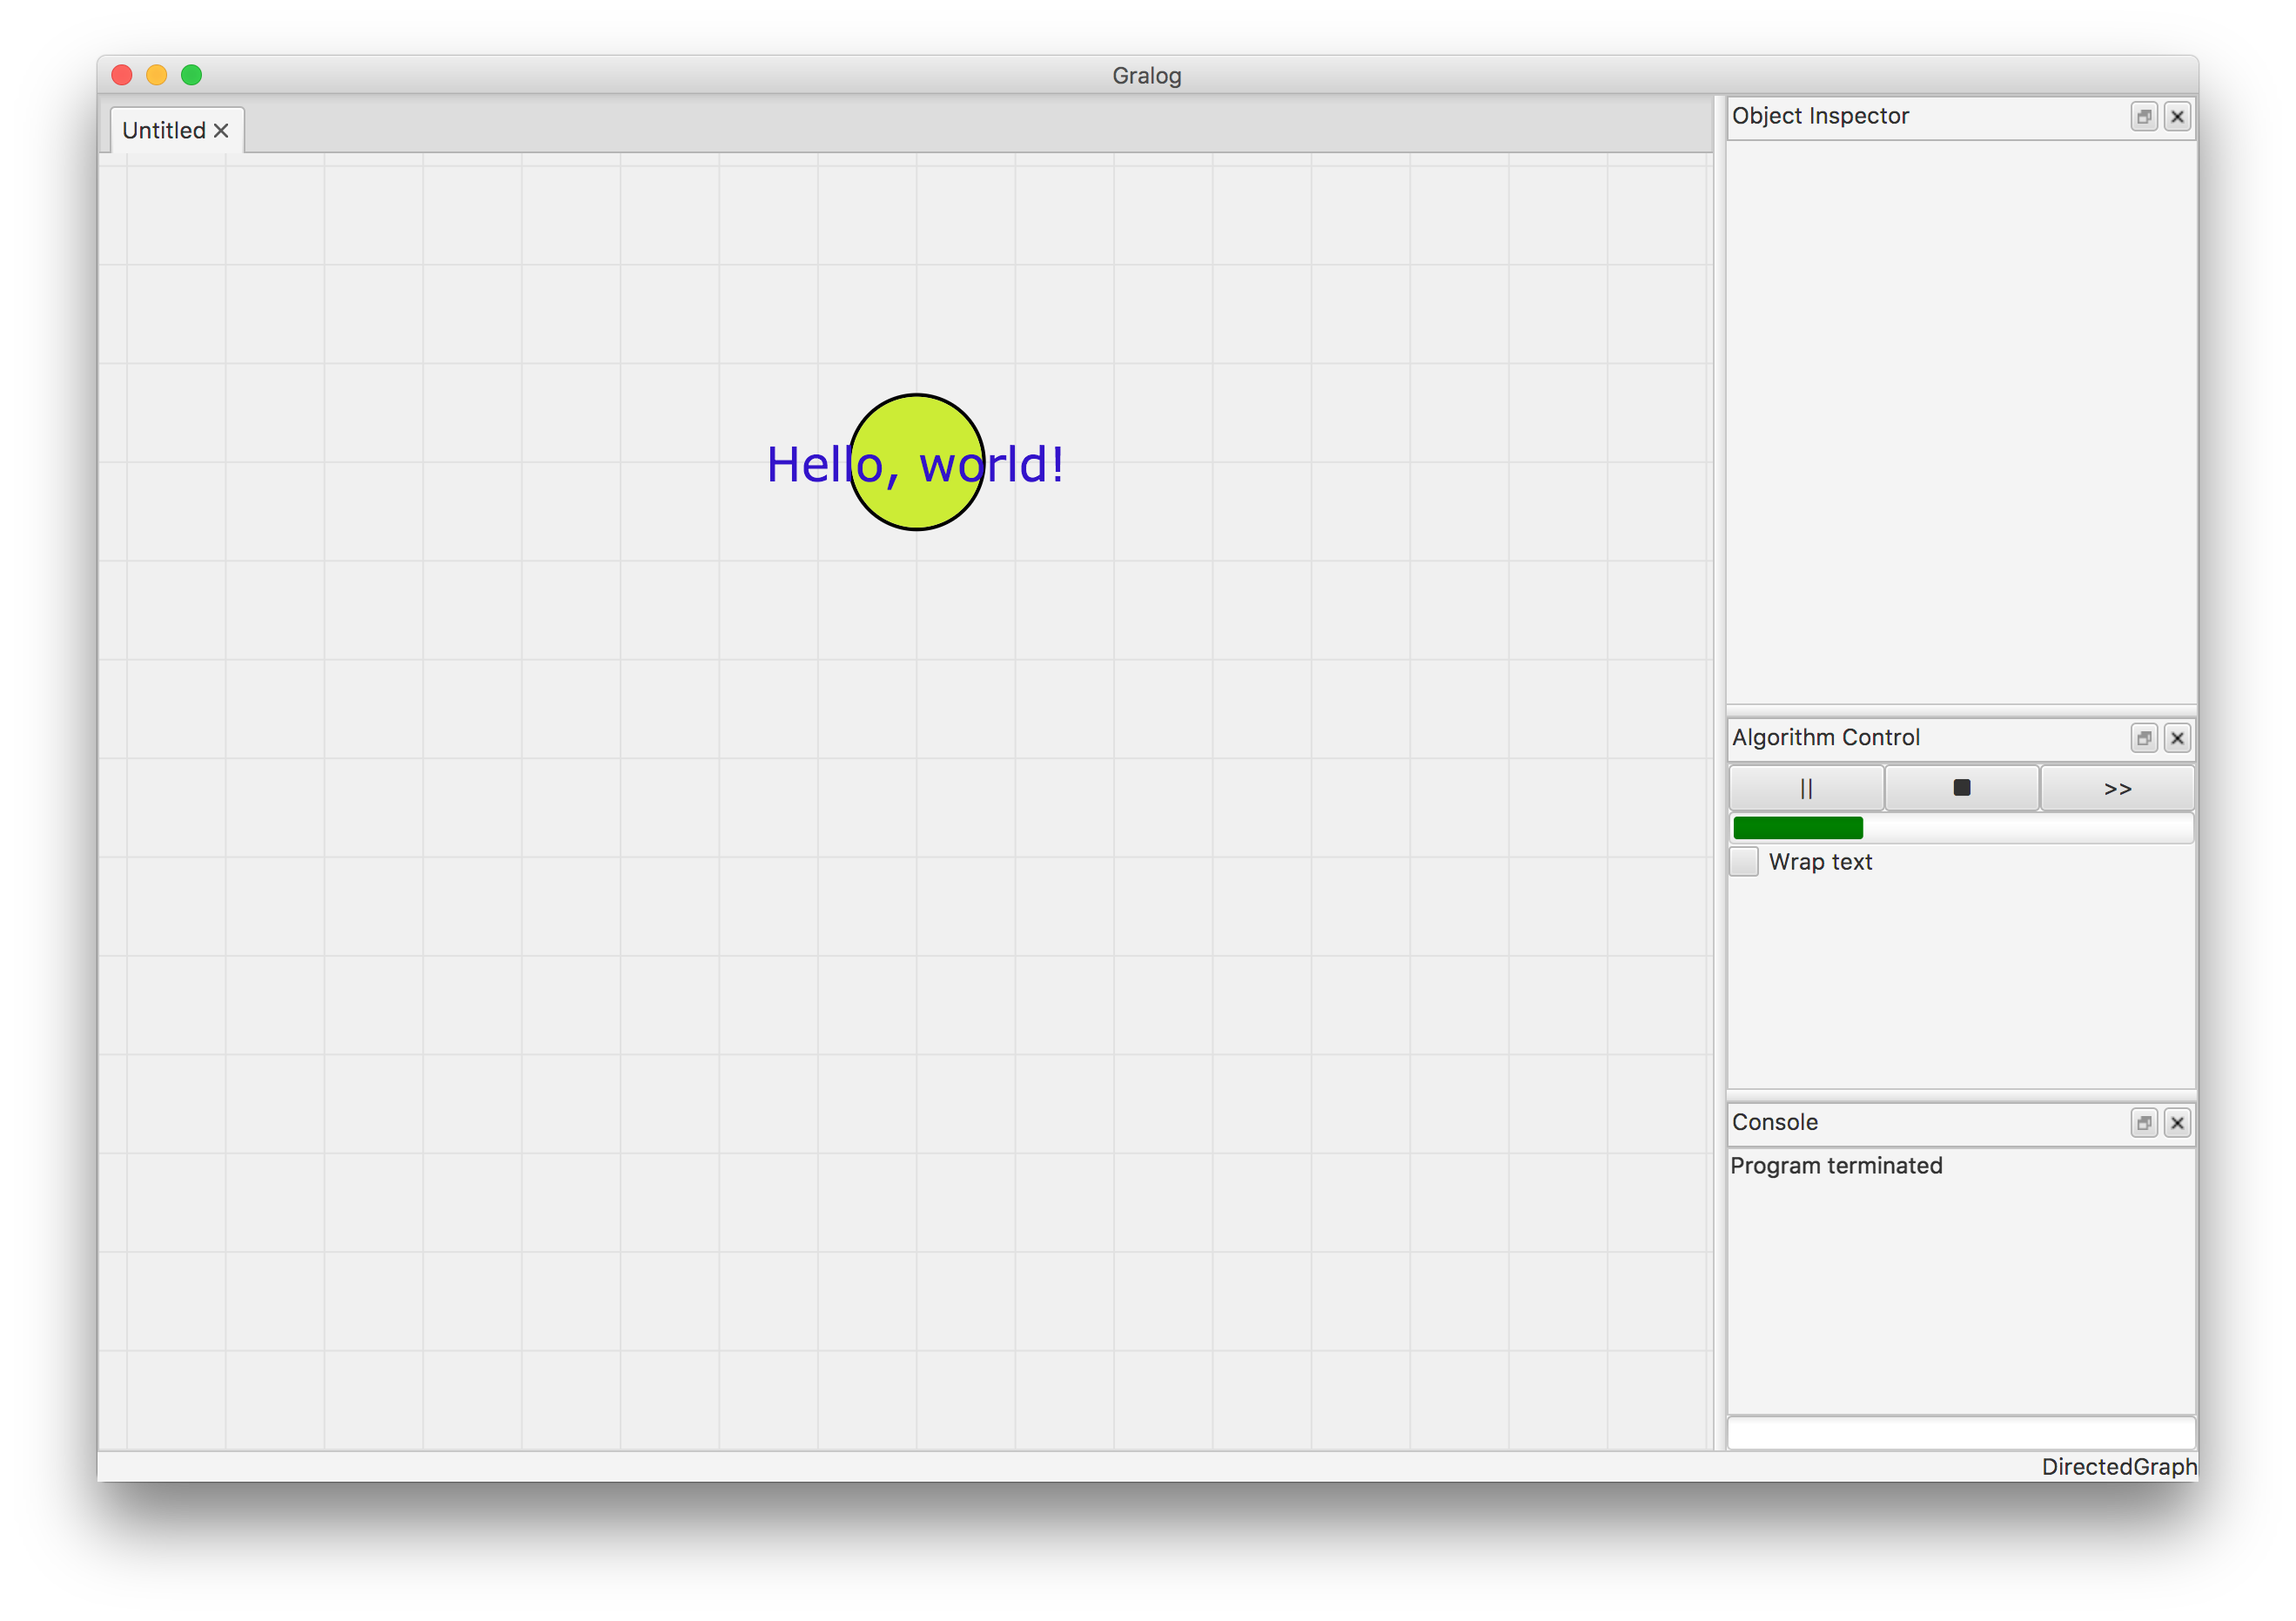
\includegraphics[width=\textwidth]{helloWorld.png}
\end{figure}

\subsection{Troubleshooting}
First obviously make sure you have python installed (version 2.7). Also make sure that Lib.py is in the directory as the file you wish to execute. Obviously you can mess around with the file structure to fit your needs but in this configuration they must be in the same directory. For other outstanding problems feel free to shoot an email at felix.herron@gmail.com 

\section{Introduction}
Now that you have the code running and set up, what will follow is a brief explanation of all of the functionality which we have built, structured in an intuitive manner.

\subsection{The Graph Class}
The first relevant class is Graph. In every program, you must choose a graph on which to execute your program. This is accomplished by instantiating the class Graph. 

\begin{lstlisting}
g = Graph();
\end{lstlisting}

In the constructor you specify which type of graph you would like. No argument means use the graph that is currently opened, whatever (type) it may be.

The Graph class can be seen as the moderator of the program. You will use it to do all of the surface-level, more general commands pertaining to the graph itself. The more intricate details will be done using the following two:

\subsection{The Vertex Class}
Each vertex is represented as an object of the class Vertex. It is distinguished by its unique ID. 

\begin{lstlisting}
v = g.createVertex();
\end{lstlisting}

All methods pertaining to the individual vertices, such as their color, neighbours, or label, are most easily manipulated using methods of this class. For example:

\begin{lstlisting}
v = g.createVertex(id=42);
v.setLabel("f00");
neighbours = v.getNeighbours();
myLabel = v.getLabel();
v.delete();
\end{lstlisting}

\subsection{The Edge Class}
Each edge is represented as an object of hte Edge class. It is distinguished by its unique ID; however, in graphs without multi-edges, it can also be distinguished by its source and target vertices.

\begin{lstlisting}
e = g.createEdge(v1,v2,directed=False);
\end{lstlisting}

All methods pertaining to the individual edges, such as their color, adjacent edges, or label, are most easily manipulated using methods of this class. For example:

\begin{lstlisting}
e = g.createEdge(v1,v2,directed=False,id=451);
e.setLabel("f00");
adjacentEdges = e.getAdjacentEdges();
target = e.getTarget();
e.delete();
\end{lstlisting}

The documentation will now simply elaborate on these concepts.

\section{Documentation}

\subsection{Class Graph}

\textbf{{\large Instance Variables}}


\begin{longtable}{p{\q}p{\q}}
Instance Variable & Meaning and Usage \\ \hline
\textbf{Dictionary} \textit{vertices} & A dictionary that holds all of the Vertex objects known to the graph. This should ideally not be changed by the programmer \\\hline
\textbf{Dictionary} \textit{edges} & A dictionary that holds all of the Edge objects known to the graph. This should ideally not be changed by the programmer \\\hline
\textbf{Integer} \textit{id} & The id of the graph that is used in communication with gralog. This should ideally not be changed by the programmer \\ \hline
\textbf{Dictionary} \textit{variablesToTrack} & Objects in format (name,value). These are displayed in the Algorithm Control Panel during pauses. These may be changed \\ \hline
\textbf{Dictionary} \textit{variablesToTrack} & Objects in format (name,value). These are displayed in the Algorithm Control Panel during pauses. These may be changed \\ \hline
\end{longtable}


\textbf{{\large Relevant Methods}}
\textit{Note: optional parameters are in parentheses}


\begin{longtable}{m{\smallCol}m{\argsLen}m{\smallCol}m{\q}}
Method & Arguments & Returns & Description \\ \hline
\textbf{Graph}& (str: format) & Graph Object & Returns a graph object. The parameter options are either nothing, ``directed'',``undirected'',``buechi'',``kripke'',``automaton'' \\\hline
\\\multicolumn{4}{c}{\textbf{Graph Manipulating Methods}}\\\\\hline
\textbf{addVertex}  & \makecell{(int: x)\\(int: y)\\(int: vertexId)} & \textbf{Vertex} object & creates a new Vertex object. If no coordinates passed, random coordinates are chosen. If no id is passed, a suitable id is chosen. If an id is passed that has already been assigned, a suitable new one is chosen\\\hline
\textbf{deleteVertex} & Vertex Object or id of vertex & void & Deletes the vertex or the vertex with the given id from the graph\\ \hline
\textbf{addEdge} & \makecell{Vertex: sourceVertex\\Vertex: targetVertex\\(Boolean: directed) \\ (int: edgeId)} & \textbf{Edge} object & creates a new Vertex object from the source vertex to the target vertex. If directed is not specifeed, un-directed is assumed. If un-directed, the order of target and source vertex is irrelevant. If no id is passed, a suitable id is chosen. If an id is passed that has already been assigned, a suitable new one is chosen \\ \hline
\textbf{addDirectedEdge} & \makecell{Vertex: sourceVertex\\Vertex: targetVertex \\ (int: edgeId)} & \textbf{Edge} object & calls addEdge with directed=True \\ \hline
\textbf{deleteEdge} & Edge object or id of edge & void &  Deletes the edge or the edge with the given id from the graph\\ \hline
\textbf{deleteAllEdges} & (Vertex,Vertex): source, target & void & removes all directed edges from start to target, as well as all un-directed edges from between the two vertices \\ \hline
\\\multicolumn{4}{c}{\textbf{Setter Functions}}\\\\\hline
\textbf{setVertexFillColor} & \makecell{Vertex: vertex\\(str: colorHex)\\(int,int,int): colorRGB)} & void & sets the \textit{fill} color of the given vertex to the Hex code color specified or the RGB color specified. colorHex can also be a string of a common collor, such as "red" or "green."  \\ \hline
\textbf{setVertexStrokeColor} & \makecell{Vertex: vertex\\(str: colorHex)\\(int,int,int): colorRGB)} & void & sets the \textit{stroke} color of the given vertex to the Hex code color specified or the RGB color specified. colorHex can also be a string of a common collor, such as "red" or "green."  \\ \hline
\textbf{setEdgeContour} & \makecell{Edge: edge\\str: contour} & void & sets the \textit{contour} color of passed edge. Possible values are ``dashed",``dotted",``plain" \\ \hline
\textbf{setEdgeColor} & \makecell{Edge: edge\\(str: colorHex)\\((int,int,int): colorRGB)} & void & sets the color of the given edge to the Hex code color specified or the RGB color specified. colorHex can also be a string of a common collor, such as "red" or "green."  \\ \hline
\textbf{setVertexRadius} & \makecell{Vertex: vertex\\float: radius} & void & sets the radius of the given vertex to the radius specified  \\ \hline
\textbf{setVertexHeight} & \makecell{Vertex: vertex\\float: height} & void & sets the height of the given vertex to the height specified  \\ \hline
\textbf{setVertexWidth} & \makecell{Vertex: vertex\\float: width} & void & sets the width of the given vertex to the height specified  \\ \hline
\textbf{setVertexDimension} & \makecell{Vertex: vertex\\float: width\\str: dimension} & void & sets the dimension of the given vertex to the dimension specified. This functionality is primarily useful for non-standard shapes, if you were to extend gralog to include such a thing. \\ \hline
\textbf{setVertexShape} & \makecell{Vertex: vertex\\str: shape} & void & sets the given vertex to be the specified shape. Currently supported are ``ellipse,",``diamond", and ``rectangle"  \\ \hline
\textbf{setEdgeWeight} & \makecell{Edge: edge\\float: weight} & void & sets edge weight (ie. thickness) to be as wide as you specified  \\ \hline
\end{longtable}




\end{document}

